\newpage
\section{Metodo Perona-Malik}

Il metodo Perona-Malik, come anticipato, si basa sull'equazione del calore. L'idea è quella di applicare tale equazione lontano dai bordi dell'immagine e mantenere invece inalterati quest'ultimi.
Questo metodo risulta particolarmente efficace per risolvere problemi di disturbo come ad esempio un rumore del tipo salt and pepper, cioè con dei pixel bianchi o neri sparsi per la foto.\\
\vspace{1em}
\`E bene capire da un punto di vista prettamente matematico cosa vuol dire che il metodo si basa sull'equazione del calore, che ricordiamo essere:\\
$$
\begin{cases}
\frac{\partial u}{\partial t}(t,x)-\Delta u(t,x) = 0 \ x \in \mathbb R^2, t\ge 0 \ .\\ 
u(0,x) = u_0(x)\ . \\
\end{cases}
$$
Il laplaciano è la divergenza del gradiente, ed è qui che viene operata la modifica.\\
Come detto: $\Delta(u)=div(\nabla(u))$, volendo operare un controllo si introdurrà un coefficiente $k$ ottenendo $div(k\nabla(u))$, nel caso esso sia uno scalare costante, avremo $div(k\nabla(u))=kdiv(\nabla(u))=k\Delta(u)$ ed è il caso implementato nelle pagine precedenti. Il metodo Perona-Malik invece prevede l'impiego di un coefficiente k non costante, ma che cambi a seconda del pixel su cui si opera, otteniamo così una matrice delle stesse dimensioni della matrice che rappresenta l'immagine e che funga da mappa, indicante per ogni pixel l'intensità con cui la diffusione va applicata. In questo senso, questo filtro viene detto di diffusione anisotropa.
Il termine diffusione anisotropa indica, a livello globale, quella particolare proprietà secondo cui la diffusione del colore sull'immagine dipende fortemente dalla direzione presa in considerazione. Tuttavia è possibile constatare come questa dicitura sia in realtà un abuso di notazione di cui ci serviamo in termini prettamente esplicativi dal momento che il metodo in esame è localmente isotropo, si articola cioè lungo un’unica direzione variandone però l’intensità punto per punto.
%Il termine anisotropo indica come la diffusione sia diversa nelle varie direzioni, capiamo quindi come questa notazione, per quanto esplicativa sia in verità un abuso di notazione siccome la diffusione non avviene in direzioni diverse ma semplicemente con intensità diverse.
Esistono tuttavia dei metodi metodi di diffusione anisotropa, in tal caso k sarà un tensore variabile.\\
\vspace{1em}
Ritornando al metodo in esame, il problema affrontato diventa\\
$$
\begin{cases}
\frac{\partial u}{\partial t}(t,x)-div(k\nabla(u)) = 0 \ x \in \mathbb R^2, t\ge 0 \ .\\ 
\frac{\partial u}{\partial N}=0 \ x \in \mathbb R^2, t\ge 0 \ .\\ 
u(0,x) = u_0(x)\ . \\
\end{cases}
$$
Con k dipendente dal gradiente, in particolare $k=k(|\nabla(u)|^2)$.

Servirà dunque esplicitare e discretizzare questo problema, per fare ciò saranno impiegati, oltre ai metodi già visti, altri accorgimenti.\\

\newpage
\subsection{Soluzione discreta della PDE}
Sia u una funzione, sia $D_f(x_i)$ la differenza finita in avanti, $D_b(x_i)$ la differenza finita all'indietro e sia $D_c(x_i)$ la differenza finita centrata, si può osservare che:
$$
D_f(x_i)+D_b(x_i)= \frac{u_{i+1} - u_{i}}{\Delta(x)} + \frac{u_{i} - u_{i-1}}{\Delta(x)} = \frac{u_{i+1} - u_{i-1}}{\Delta(x)} = 2D_c(x_i)
$$
Capiamo quindi che la differenza finita centrata è $D_c(x_i)=\frac{1}{2}(D_f(x_i)+D_b(x_i))$ cioè la media delle altre due.\\ Preso un punto si può operare le differenze finite nelle 4 direzioni, le indicheremo con N (Nord), S (Sud), W (Ovest) e E (Est). Notiamo allora che la differenza finita Nord è la differenza finita in avanti rispetto a y, mentre la differenza finita S è la differenza finita all'indietro rispetto a y, la loro media sarà quindi la differenza finita centrata rispetto a y. Analogamente la media delle differenze finite Ovest ed Est sarà la differenza finita centrata rispetto a x. In formule:\\
%\vspace{-1em}
$$
\frac{\partial u}{\partial x} \approx \frac{u_E+u_W}{2} \hspace{1em};\hspace{1em}
\frac{\partial u}{\partial y} \approx \frac{u_N+u_S}{2}
$$
Ricordiamo che il gradiente è il vettore delle derivate parziali, la divergenza invece è la somma delle derivate parziali.
Calcoliamo quindi un'approssimazione discreta della PDE\\
%\vspace{-1em}


\begin{align*}
    \frac{\partial u}{\partial t}(t,x)&=div(k\nabla(u))=\\
    &=\frac{k\nabla u}{\partial x} +\frac{k\nabla u}{\partial y}\\
    &\approx\frac{k_N\nabla_N + k_S\nabla_S}{2} +\frac{k_W\nabla_W + k_E\nabla_E}{2}\\
    &=\frac{1}{2}(k_N\nabla_N + k_S\nabla_S k_W\nabla_W + k_E\nabla_E) 
\end{align*}


Ci si ritrova quindi a risolvere l'equazione 
$$
\frac{\partial u}{\partial t}(t,x)=\frac{1}{2}(k_N\nabla_N + k_S\nabla_S k_W\nabla_W + k_E\nabla_E) 
$$
che è della forma $y'(x)=f(x,y(x))$ e può quindi essere risolta con un metodo semplice.
Ancora una volta ricorriamo alle differenze finite.
$$
y'(x_i)\approx \frac{y(x_{i+1})-y(x_{i})}{\Delta t} 
$$
ma $y'(x)=f(x,y(x))$ questo vuol dire che
$$
\frac{y(x_{i+1})-y(x_{i})}{\Delta t}\approx f(x,y(x)) \Rightarrow y_{i+1} \approx y_{i} + \Delta t f(x,y(x))
$$
tale metodo è detto \textbf{metodo di Eulero esplicito}\footnote{\cite{monegato}}

La soluzione discreta della PDE, con il metodo di Eulero esplicito, sarà quindi:\\

$$
u_{i+1} = u_i + dt\frac{1}{2}(k_N\nabla_N + k_S\nabla_S + k_W\nabla_W + k_E\nabla_E)
$$

%\subsubsection{Stabilità del metodo}
\begin{osservazione}
Tramite il metodo di Von Neuman, in modo simile a quanto fatto per l'equazione del calore si
dimostra che il metodo Perona-Malik risulta essere\\
\vspace{0.25em}
stabile $\Longleftrightarrow 4\frac{1}{2}\frac{dt}{\Delta x^2}\leq\frac{1}{2}$.\\
\vspace{0.25em}
Ricordiamo che nel caso in esame, ove $\Delta x=1$, la condizione diventa:
$$
dt\leq \frac{1}{4}.
$$
\end{osservazione}


\subsection{Maschere di convoluzione}
Per implementare il filtro di diffusione anisotropica detto \textit{Perona-Malik}, ci serviremo di alcune \textbf{maschere}.\\
Un filtro è una funzione $F:\mathbb R^2\to\mathbb R$,
%in quanto tale avrà un nucleo $\operatorname{Ker}(F):=\{v \in \mathbb R^2: Fv=0\}$ che 
in particolare è un polinomio a due incognite che, date in input delle coordinate restituirà un valore numerico, chiameremo tale coefficiente \textbf{peso}. Compiliamo quindi una maschera con i pesi calcolati in tal modo per ogni posizione ottenendo una cosa del tipo:

\begin{figure}[]
    \centering
    \begin{tabular}{|p{1.6cm}|p{1.6cm}|p{1.6cm}|}
        \hline
        \makebox[1.6cm][c]{
        \rule[-8mm]{0cm}{1.6cm}
        $a_1$} & 
        \makebox[1.6cm][c]{
        $a_2$} & 
        \makebox[1.6cm][c]{
        $a_3$} \\
        \hline
        \makebox[1.6cm][c]{
        \rule[-8mm]{0cm}{1.6cm}
        $a_4$} & 
        \makebox[1.6cm][c]{
        $a_5$} & 
        \makebox[1.6cm][c]{
        $a_6$} \\
        \hline
        \makebox[1.6cm][c]{
        \rule[-8mm]{0cm}{1.6cm}
        $a_7$} & 
        \makebox[1.6cm][c]{
        $a_8$} & 
        \makebox[1.6cm][c]{
        $a_9$} \\
        \hline
    \end{tabular}
    \caption{Esempio di maschera di convoluzione 3x3}
    \label{fig:my_label}
\end{figure}
Le dimensioni della maschera possono variare a discrezione del programmatore ma, solitamente si utilizzano maschere dimensioni piccole e dispari. Dispari perchè è importante individuare il centro della maschera. Piccole perchè l'utilizzo delle maschere porta degli effetti bordo che è bene limitare. Queste motivazioni verranno meglio spiegate a breve.\\
\vspace{1em}
Come detto nelle nozioni introduttive, applicare un filtro vuol dire operare una convoluzione tra due funzioni: l'immagine ed il filtro stesso.\\
Le maschere sono un utile strumento proprio per il calcolo delle convoluzioni, motivo per cui sono solitamente dette \textbf{maschere di convoluzione}.\\
Per operare una convoluzione, detti $u:\mathbb R^2\to\mathbb R$ l'immagine e $F:\mathbb R^2\to\mathbb R$ il filtro, per definizione, $\forall p_{i,j}\in dom(u)$ si prende un intorno $I(p)$, le cui dimensioni dipendono da quelle della maschera scelta per F. Successivamente si sommano i prodotti tra i valori di u e quelli di F, cioè i pesi della maschera, per ottenere in fine l'immagine filtrata.\\
\vspace{1em}
In pratica, si scorre la maschera sui vari pixel dell'immagine\\
\begin{figure}[h!]
    \centering
    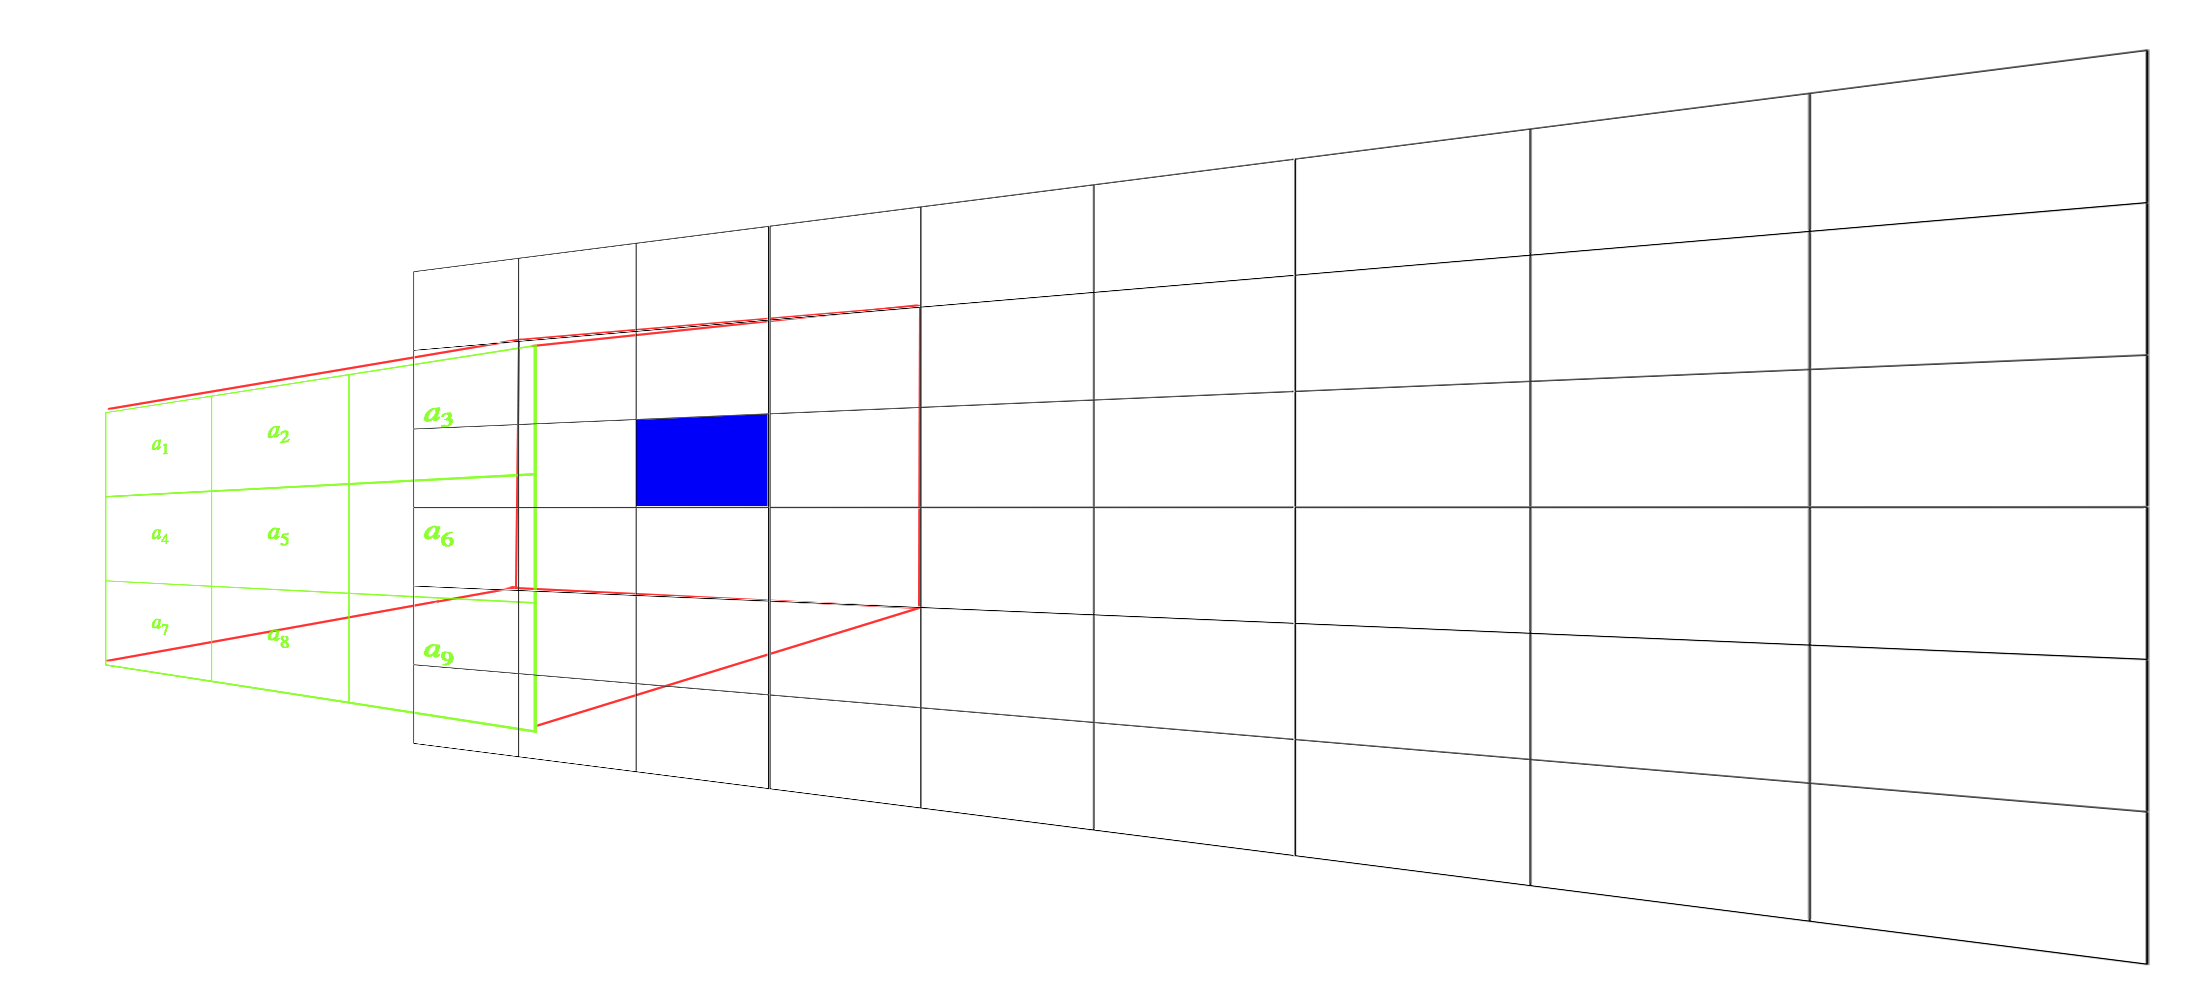
\includegraphics[scale=0.15]{Pictures/illustrazione convoluzione.png}
    \caption{Griglia dell'immagine in nero, maschera in verde, pixel in esame in blu}
    \label{fig:my_label}
\end{figure}
Per ogni pixel ne viene ricalcolato il valore come segue
\begin{figure}
    \centering
    %\begin{tabular}{|c|c|c|}
    \begin{tabular}{|p{1.6cm}|p{1.6cm}|p{1.6cm}|}
        \hline
        \makebox[1.6cm][c]{
        \rule[-8mm]{0cm}{1.6cm}
        $p_{i-1,j+1}$} & 
        \makebox[1.6cm][c]{
        $p_{i,j+1}$} & 
        \makebox[1.6cm][c]{
        $p_{i+1,j+1}$} \\
        \hline
        \makebox[1.6cm][c]{
        \rule[-8mm]{0cm}{1.6cm}
        $p_{i-1,j}$} & 
        \makebox[1.6cm][c]{
        $p_{i,j}$} & 
        \makebox[1.6cm][c]{
        $p_{i+1,j}$} \\
        \hline
        \makebox[1.6cm][c]{
        \rule[-8mm]{0cm}{1.6cm}
        $p_{i-1,j-1}$} & 
        \makebox[1.6cm][c]{
        $p_{i,j-1}$} & 
        \makebox[1.6cm][c]{
        $p_{i+1,j-1}$} \\
        \hline
    \end{tabular}
    \hspace{1em}
    \huge{*}
    \normalsize
    \hspace{1em}
    \begin{tabular}{|p{1.6cm}|p{1.6cm}|p{1.6cm}|}
        \hline
        \makebox[1.6cm][c]{
        \rule[-8mm]{0cm}{1.6cm}
        $a_1$} & 
        \makebox[1.6cm][c]{
        $a_2$} & 
        \makebox[1.6cm][c]{
        $a_3$} \\
        \hline
        \makebox[1.6cm][c]{
        \rule[-8mm]{0cm}{1.6cm}
        $a_4$} & 
        \makebox[1.6cm][c]{
        $a_5$} & 
        \makebox[1.6cm][c]{
        $a_6$} \\
        \hline
        \makebox[1.6cm][c]{
        \rule[-8mm]{0cm}{1.6cm}
        $a_7$} & 
        \makebox[1.6cm][c]{
        $a_8$} & 
        \makebox[1.6cm][c]{
        $a_9$} \\
        \hline
    \end{tabular}
    \small{
    $$
    u(p_{i,j})*F=a_1p_{i-1,j+1} + a_2p_{i,j+1} + a_3p_{i+1,j+1} + a_4p_{i-1,j} + a_5p_{i,j} + a_6p_{i+1,j} + a_7p_{i-1,j-1} + a_8p_{i,j-1} + a_9p_{i+1,j-1}.
    $$
    }\\
\caption{Intorno di un punto, maschera di convoluzione e soluzione analitica}
\label{fig:my_label}
\end{figure}

\vspace{-1em}

Ma allora una convoluzione con $a=$
    \begin{tabular}{|p{0.4cm}|p{0.4cm}|p{0.4cm}|}
        \hline
        \makebox[0.4cm][c]{
        \rule[-2mm]{0cm}{0.6cm}
        $0$} & 
        \makebox[0.4cm][c]{
        $1$} & 
        \makebox[0.4cm][c]{
        $0$} \\
        \hline
        \makebox[0.4cm][c]{
        \rule[-2mm]{0cm}{0.6cm}
        $0$} & 
        \makebox[0.4cm][c]{
        $-1$} & 
        \makebox[0.4cm][c]{
        $0$} \\
        \hline
        \makebox[0.4cm][c]{
        \rule[-2mm]{0cm}{0.6cm}
        $0$} & 
        \makebox[0.4cm][c]{
        $0$} & 
        \makebox[0.4cm][c]{
        $0$} \\
        \hline
    \end{tabular}
\vspace{0.5em}
vuol dire fare la derivata prima approssimata alle differenze finite lungo y, in particolare verso l'alto, infatti facendo il conto di cui sopra si ottiene $u(p_{i,j})*F=p_{i,j+1}-p_{i,j}$ che è esattamente quanto trovato analizzando il metodo alle differenze finite
si può operare analogamente in tutte e 4 le direzioni.\\
\vspace{1em}
Per facilitare la successiva implementazione del filtro, si è scritta una funzione MATLAB che operi in tal senso.

\begin{lstlisting}[language=MATLAB]
function B=convoluzione(A,k);

[r c] = size(A);            %Memorizzo le dimensioni dell'immagine
[m n] = size(k);            %Memorizzo le dimensioni della maschera
h = rot90(k, 2);

%Definisco una cornice per gestire gli effetti di bordo
center = floor((size(h)+1)/2);                  
left = center(2) - 1;
right = n - center(2);
top = center(1) - 1;
bottom = m - center(1);

%Preparo un "piano di lavoro"
Rep = zeros(r + top + bottom, c + left + right);
for x = 1 + top : r + top
    for y = 1 + left : c + left
        Rep(x,y) = A(x - top, y - left);
    end
end

%Opero la convoluzione
B = zeros(r , c);
for x = 1 : r
    for y = 1 : c
        for i = 1 : m
            for j = 1 : n
                q = x - 1;
                w = y -1;
                B(x, y) = B(x, y) + (Rep(i + q, j + w) * h(i, j));
            end
        end
    end
end

\end{lstlisting}
Notare che \texttt{Rep} ha dimensioni maggiori rispetto all'immagine questo perchè dobbiamo gestire anche i pixel sui bordi del riquadro dell'immagine. Volendo fare un esempio, si consideri il pixel in posizione (1,1), ossia l'angolo in alto a sinistra, allora i coeff $a_1$, $a_2$, $a_3$, $a_4$ e $a_7$, non avranno nessun corrispettivo da moltiplicare, costruiamo quindi una cornice nera (cioè pixel di valore nullo) per ovviare a questo problema. Ovviamente se la maschera è grande, questo porterà a dei visibili errori di bordo, il che è esattamente il motivo per cui si usano solitamente maschere di dimensioni molto piccole.




\newpage
\subsection{Rilevamento dei bordi}
Il metodo Perona-Malik serve ad eliminare il rumore, preservando i bordi. Per essere in grado di preservarli però dobbiamo prima essere in grado di riconoscerli. Il metodo prevede l'introduzione del termine $K(\Delta(u))$ che dipende quindi dal laplaciano dell'immagine che si intende filtrare. Cerchiamo di capire il perché di questa scelta.\\
\vspace{1em}
Operando una derivata in una data direzione, per il significato in sè di derivata, questa assume valori più elevati quando la variazione è elevata, e assume valori nulli quando non c'è variazione in quella direzione. Per questo motivo, applicata ad un' immagine, ne rileviamo i bordi.\\
Presa una tinta unita la derivata sarà quindi nulla in ogni suo punto (è intuitivo: se un'immagine è una funzione che, date due coordinate restituisce un colore, allora una tinta unita è una funzione costante ed in quanto tale ha derivata nulla).\\
Operando una derivata seconda in una data direzione, per il significato in sè di derivata seconda, questa assume valori più elevati quando la concavità è più stretta, e assume valori pressocchè nulli quando non ci sono concavità (si può pensare alle concavità come a dei picchi o dei ventri, su di una immagine vuol dire chiazze di colore diverso).\\
Presa una sfumatura di colore che varia in maniera lineare, la derivata seconda sarà nulla in ogni suo punto, la derivata prima sarà invece costante.\\x
\vspace{1em}
Per verificare la validità di questi concetti teorici si è implementato un semplice script MATLAB che, presa un'immagine, opera il calcolo delle derivate e stampa a video le sole derivate sotto forma di immagine. Ne risulterà quindi un'immagine in bianco e nero con pixel quanto più chiari quanto più e alto il valore della derivata. Saranno mostrate come immagini diverse le derivate parziali, il gradiente ed il laplaciano dell'immagine data in input, così da poterli confrontare ed evidenziarne le differenze. Ci aspettiamo che le immagini risultanti corrispondano con i bordi dell'immagine originale.\\
Saranno mostrati i risultati prodotti da tale script dandogli in input immagini di diverso tipo, saranno poi commentati con osservazioni e considerazioni di vario tipo.
\newpage
Si riporta lo script MATLAB appena citato.
\vspace{1em}
\begin{lstlisting}[language=MATLAB]
%---Operazioni preliminari
Im=imread("nome_immagine.png");	%Apro l'immmagine

[ny, nx, ~]=size(Im)        %Memorizzo le dimensioni dell'immagine
u=double(Im);               %Copia dell'immagine originale su cui lavorare
h=80;                       %Definisco un parametro che usero' per                               enfatizzare i bordi in fase di stampa 


%---Calcolo tutte le derivate
u_x =  u(:,[1 1:nx-1],:) - u;                       %derivata                                                            prima lungo x
u_xx = u(:,[2:nx nx],:) - 2*u + u(:,[1 1:nx-1],:);  %derivata                                                            seconda lungo x
u_y =  u([1 1:ny-1],:,:) - u;                       %derivata                                                            prima lungo y
u_yy = u([2:ny ny],:,:) - 2*u + u([1 1:ny-1],:,:);  %derivata                                                            seconda lungo y
u_xy = u_x([1 1:ny-1],:,:) - u_x;                   %derivata                                                            seconda mista
   
%---Stampo i risultati
figure()
subplot(2,3,2),text(0.3,0,nome,'FontSize',20); axis off
subplot(2,3,4), imshow(Im)
title('Immagine originale')
subplot(2,3,5), imshow(uint8(h*abs(u_x)))
title('h*u_x')
subplot(2,3,6), imshow(uint8(h*abs(u_y)))
title('h*u_y')

figure()
subplot(2,3,2),text(0.3,0,nome,'FontSize',20); axis off
subplot(2,3,4), imshow(Im)
title('Immagine originale')
subplot(2,3,5), imshow(uint8(h*abs(u_x + u_y)))
title('h*(u_x + u_y)')
subplot(2,3,6), imshow(uint8(h*abs(u_xx + u_yy)))
title('h*(u_{xx} + u_{yy})')
\end{lstlisting}

\vspace{1em}
Eseguiamo adesso questo script che ci permetterà di osservare, fornendogli in input diverse immagini molto semplici, se abbiamo ottenuto i risultati attesi.\\
%\vspace{1em}
\newpage
\subsubsection{Esempio 1 - Tinta unita}
\begin{figure}[htb]
\centering
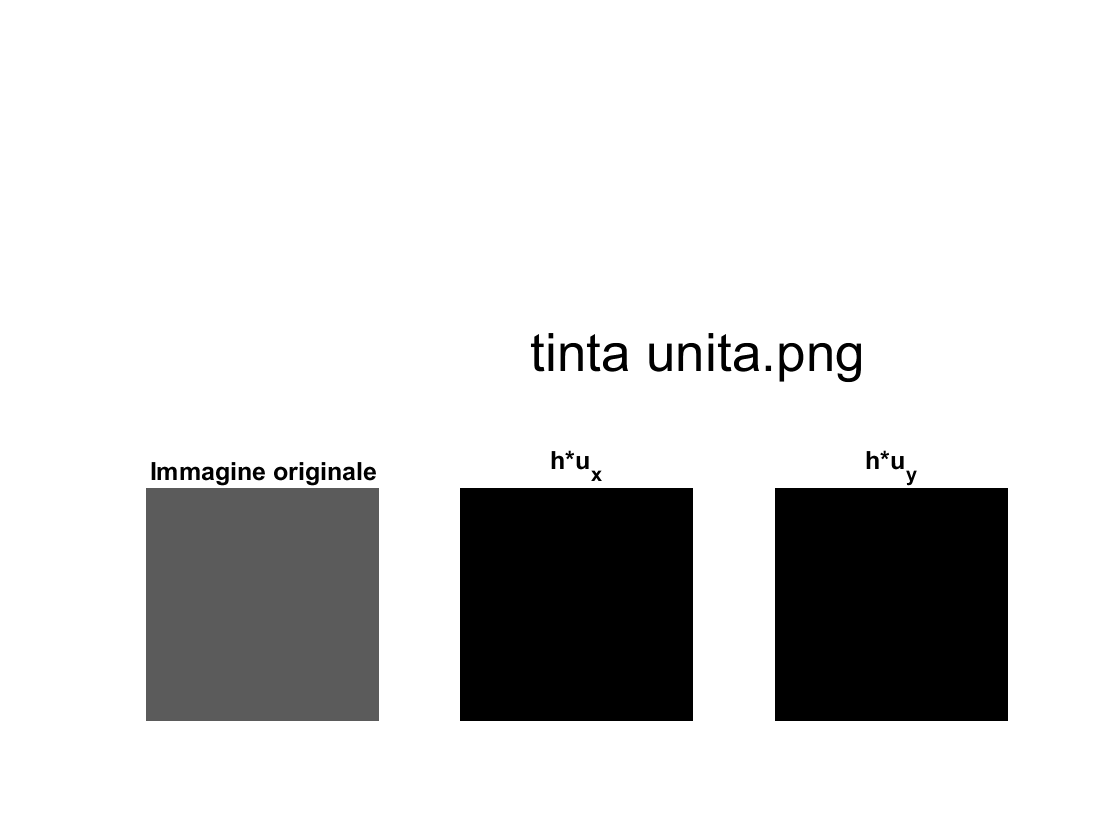
\includegraphics[scale=0.4, trim = 0 2cm 0 11.5cm, clip]{Pictures/Risultati/tinta unita bianco e nero derivate parziali.png}
%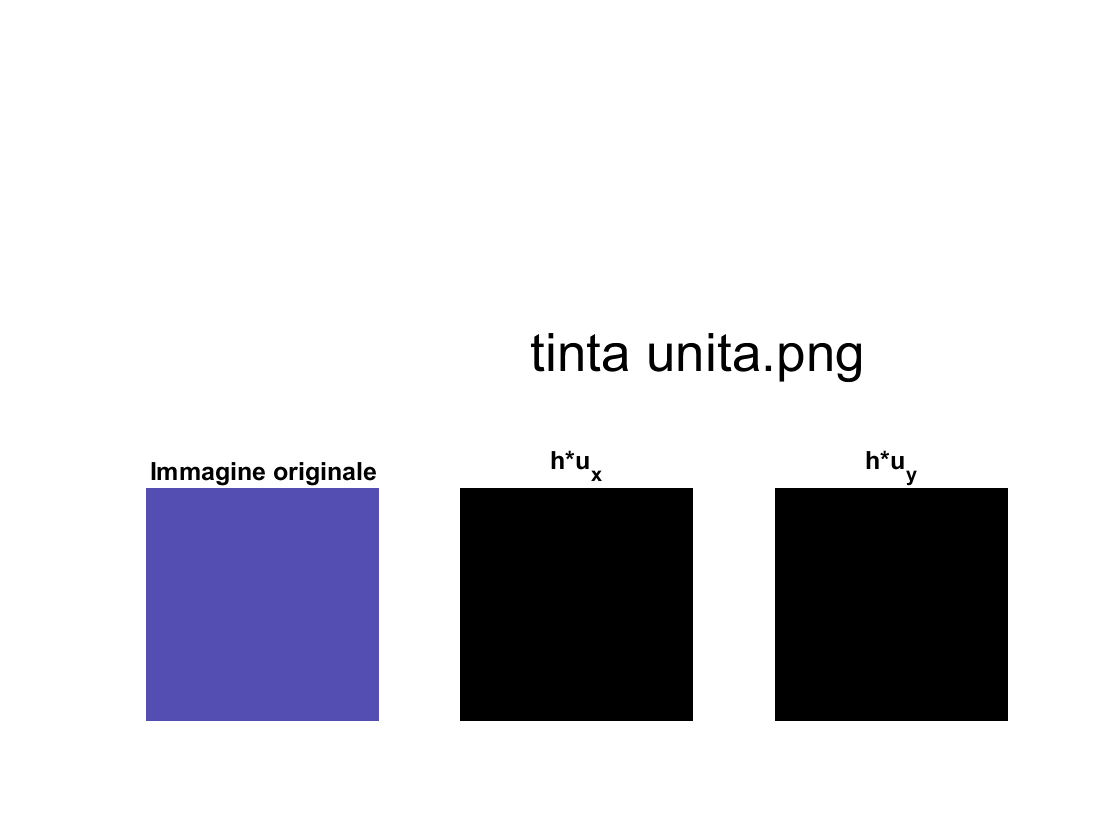
\includegraphics[scale=0.4, trim = 0 0 0 10.5cm, clip]{Pictures/Risultati/tinta unita derivate parziali.png}
\caption{Derivate parziali di una tinta unita.}\label{fig:figura}
\end{figure}

Si può vedere come con un'immagine a tinta unita le derivate sono nulle, quindi lo saranno anche gradiente e laplaciano.\\

\subsubsection{Esempio 2 - Sfumatura lungo l'asse x}
\begin{figure}[htb] 
\centering
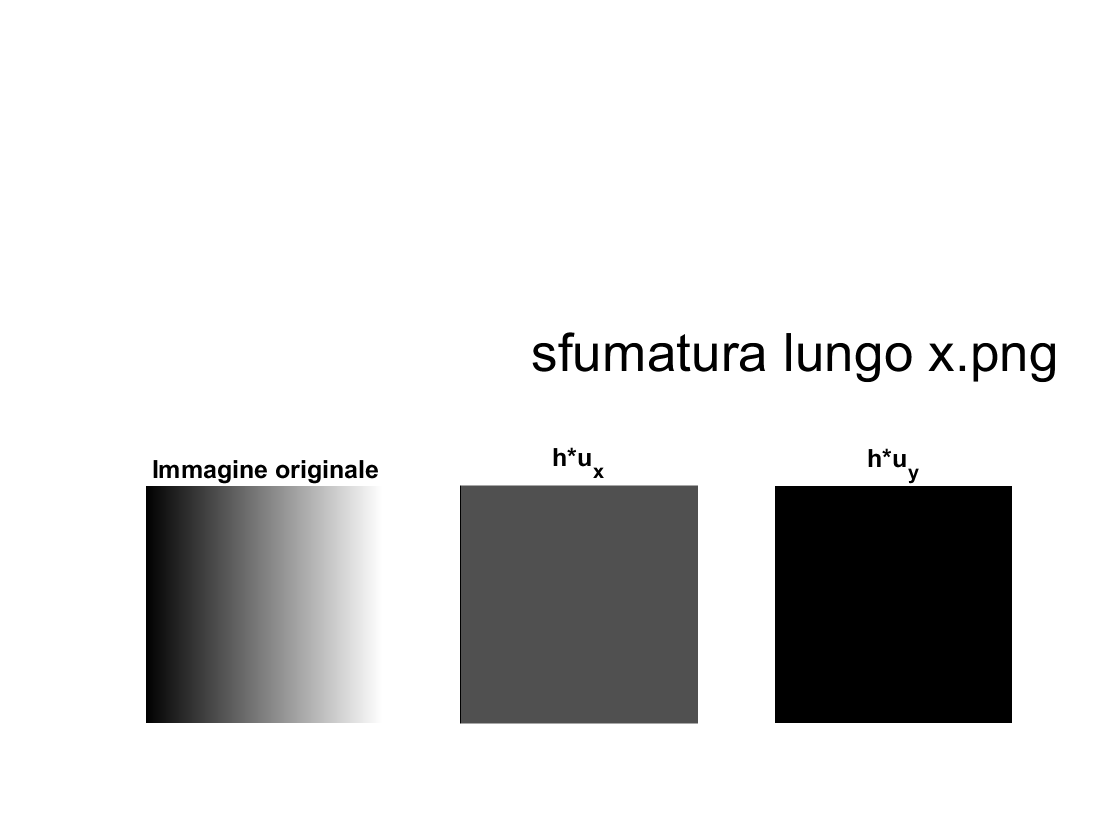
\includegraphics[scale=0.4, trim = 0 2cm 0 11.5cm, clip]{Pictures/Risultati/sfumatura lungo x bianco e nero derivate parziali.png}
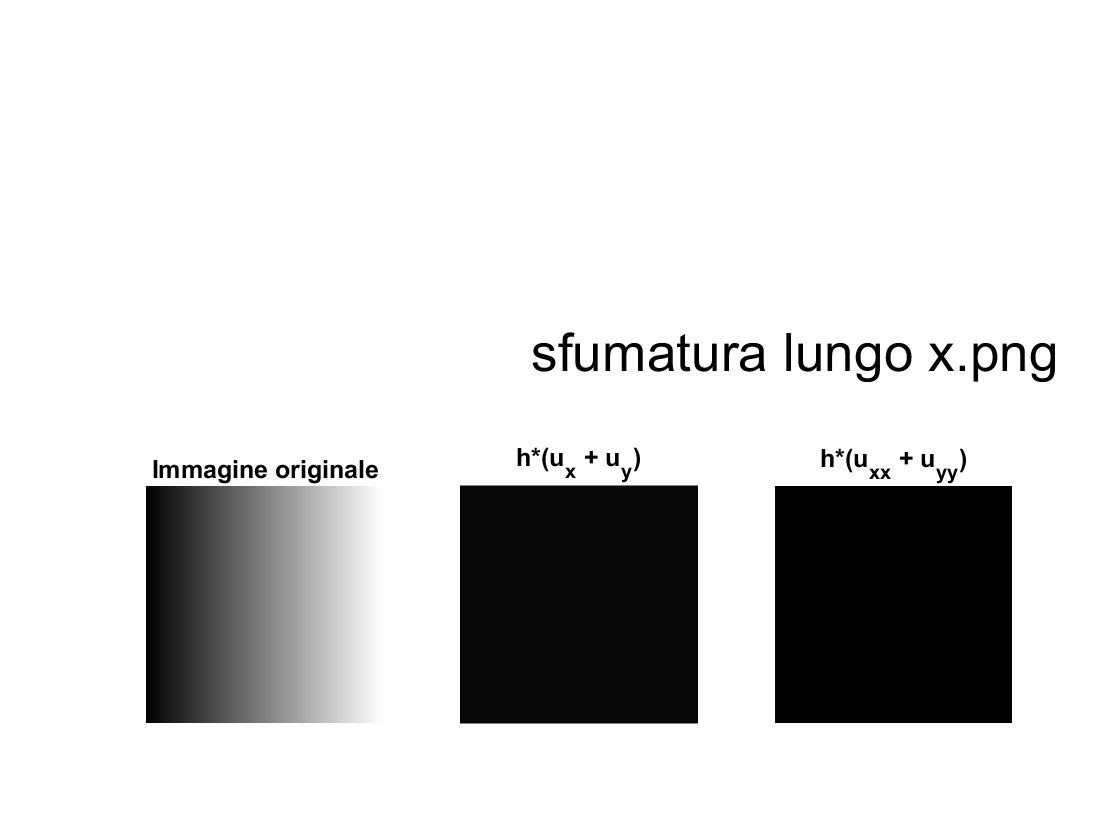
\includegraphics[scale=0.4, trim = 0 2cm 0 11.5cm, clip]{Pictures/Risultati/sfumatura lungo x bianco e nero gradiente e laplaciano.png}
\caption{Derivate parziali, gradiente e laplaciano di una sfumatura orizzontale.}\label{fig:figura}
\end{figure}

Guardando invece ad una immagine che presenta una sfumatura lineare lungo l'asse x, la derivata lungo x assume un valore costante mentre la derivata lungo y è nulla, proprio perchè lungo y non c'è variazione mentre lungo x c'è una variazione costante.\\
Ovviamente, date queste premesse, il gradiente sarà costante uguale ad $u_x$ (siccome $u_y=0$) e quindi il laplaciano sarà nullo.
Il fatto che in entrambi questi esempi il laplaciano sia nullo è un buon segno, lo useremo per rilevare i bordi ed in queste immagini non ve ne sono, quindi è giusto che il laplaciano sia nullo.\\

\newpage
\subsubsection{Esempio 3 - Parziale sfumatura lungo la diagonale}
\begin{figure}   
\centering
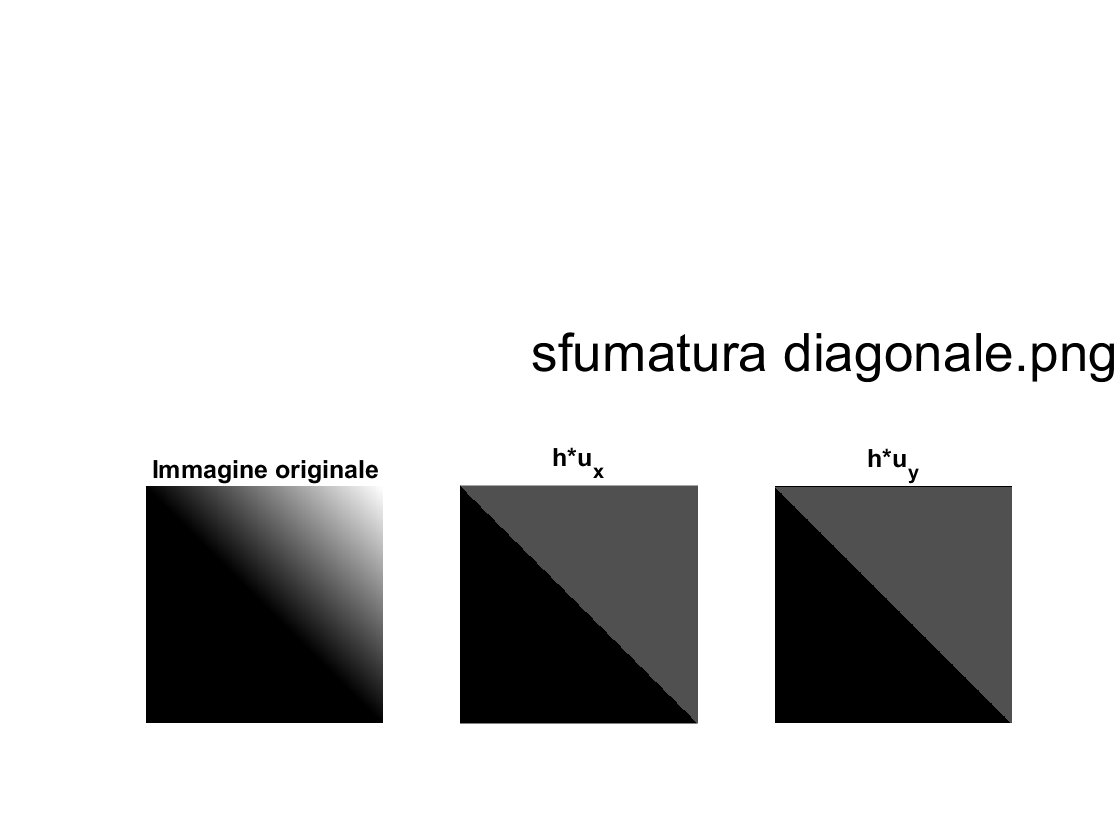
\includegraphics[scale=0.4, trim = 0 0 0 10.5cm, clip]{Pictures/Risultati/sfumatura diagonale bianco e nero derivate parziali.png}
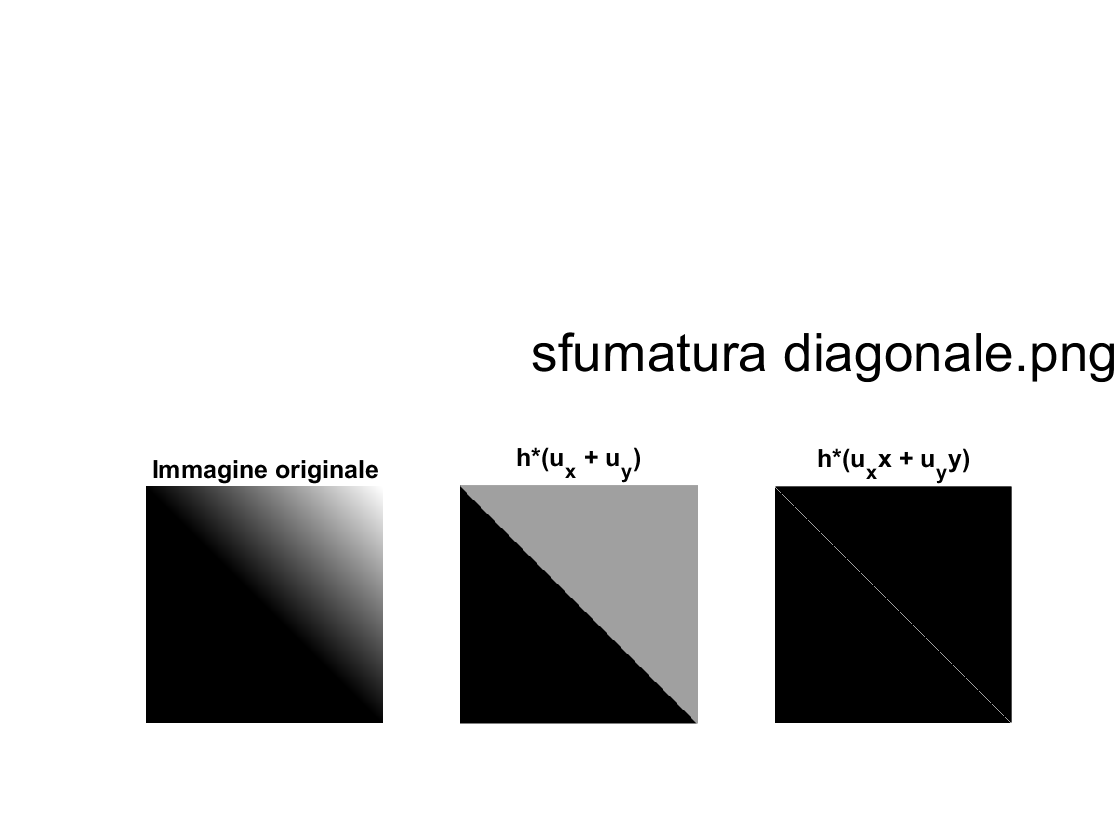
\includegraphics[scale=0.4, trim = 0 0 0 10.5cm, clip]{Pictures/Risultati/sfumatura diagonale bianco e nero gradiente e laplaciano.png}
\caption{Derivate parziali, gradiente e laplaciano di una parziale sfumatura diagonale.}\label{fig:figura}
\end{figure}

Presa una sfumatura diagonale, ma solo su metà immagine vediamo dei risultati interessanti: entrambe le derivate parziali sono nulle nelle regioni in cui non c'è sfumatura, esattamente come nel caso della tinta unita, ed entrambe sono costanti dove c'è sfumatura (che ricordiamo essere lineare).\\
Tutto ciò riconferma quanto visto dai punti precedenti, volgendo quindi uno sguardo al gradiente ed al laplaciano si può notare che mentre il gradiente ha un aspetto molto simile alle due derivate parziali, sommando i loro valori è semplicemente più luminoso, per quanto riguarda il laplaciano la storia cambia. Le derivate seconde sono indicatrici della variazione delle derivate prime, cioè della variazione della variazione del valore della funzione, ma l'unica variazione che hanno le derivate prime è lungo la diagonale.
Abbiamo così individuato il nostro primo bordo, cioè la diagonale che divide di fatto due regioni, una in cui il colore è costante ed una in cui sfuma.\\

\vspace{1em}
Si riportano ancora due varianti di un'ultima immagine esempio, provando ad introdurre una semplice figura.\\

\newpage
\subsubsection{Esempio 4 - Rettangolo bianco su sfondo nero}
\begin{figure}[htb] 
\centering
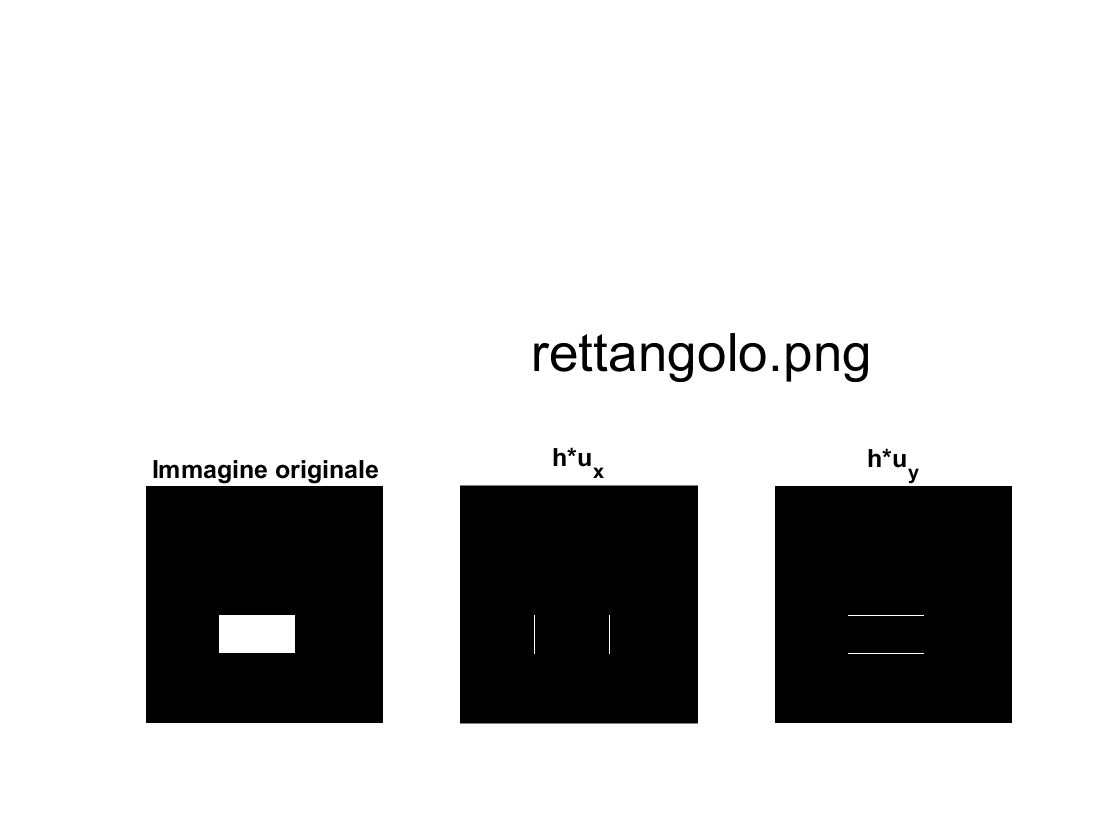
\includegraphics[scale=0.4, trim = 0 0 0 10.5cm, clip]{Pictures/Risultati/rettangolo bianco e nero derivate parziali.png}
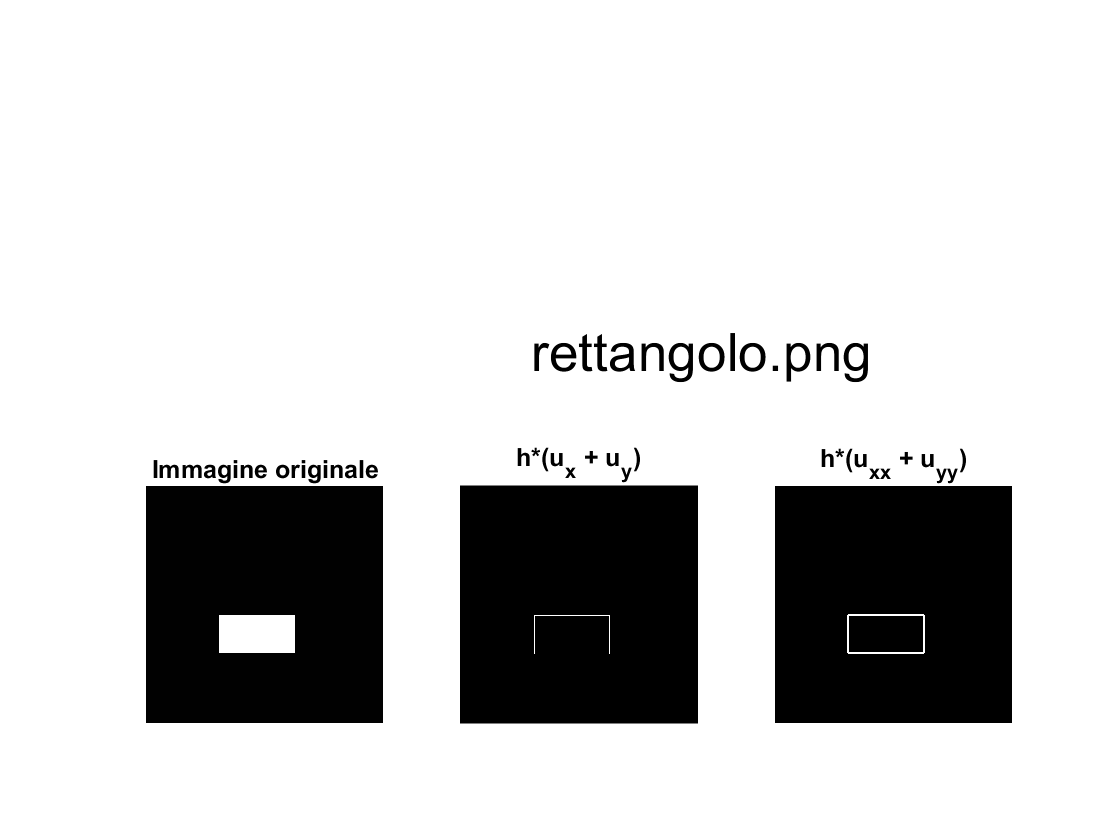
\includegraphics[scale=0.4, trim = 0 0 0 10.5cm, clip]{Pictures/Risultati/rettangolo bianco e nero gradiente e laplaciano.png}
\caption{Derivate parziali, gradiente e laplaciano di una figura semplice.}\label{fig:figura}
\end{figure}

Importando un rettangolo bianco su di uno sfondo nero, come confermato anche dalla prima sfumatura, la derivata lungo x rileva i bordi verticali, quella lungo y i bordi orizzontali, dalla loro somma (quindi dal gradiente) otteniamo già il bordo del rettangolo.
Il bordo così ottenuto è un bordo che idealmente rimarrà inalterato a prescindere dall'ordine della derivata, in particolare quindi anche per derivate seconde, quindi il laplaciano continua a soddisfare la richiesta di determinare i bordi. \\
Come detto: \textit{"Il bordo così ottenuto è un bordo che idealmente rimarrà inalterato a prescindere dall'ordine della derivata"} è interessante capire perchè. Presa una striscia di pixel, cioè uno strato dell'immagine (la si può immaginare quindi come una funzione $u_y:\mathbb{R} \longrightarrow \mathbb{R}$), risulterà essa raffigurare una funzione porta!\\
La funzione porta non è derivabile in senso classico, ripensando alla definizione di derivata avremmo un valore di +infinito prima e -infinito poi. La sua derivata sarà quindi una coppia di delta di Dirac.\\

\vspace{1em}
Proviamo in fine ad introdurre del rumore in quest'ultima immagine e osserviamo cosa accade.

\newpage
\subsubsection{Esempio 5 - Rettangolo bianco su sfondo dietro con rumore}
\begin{figure}   
\centering
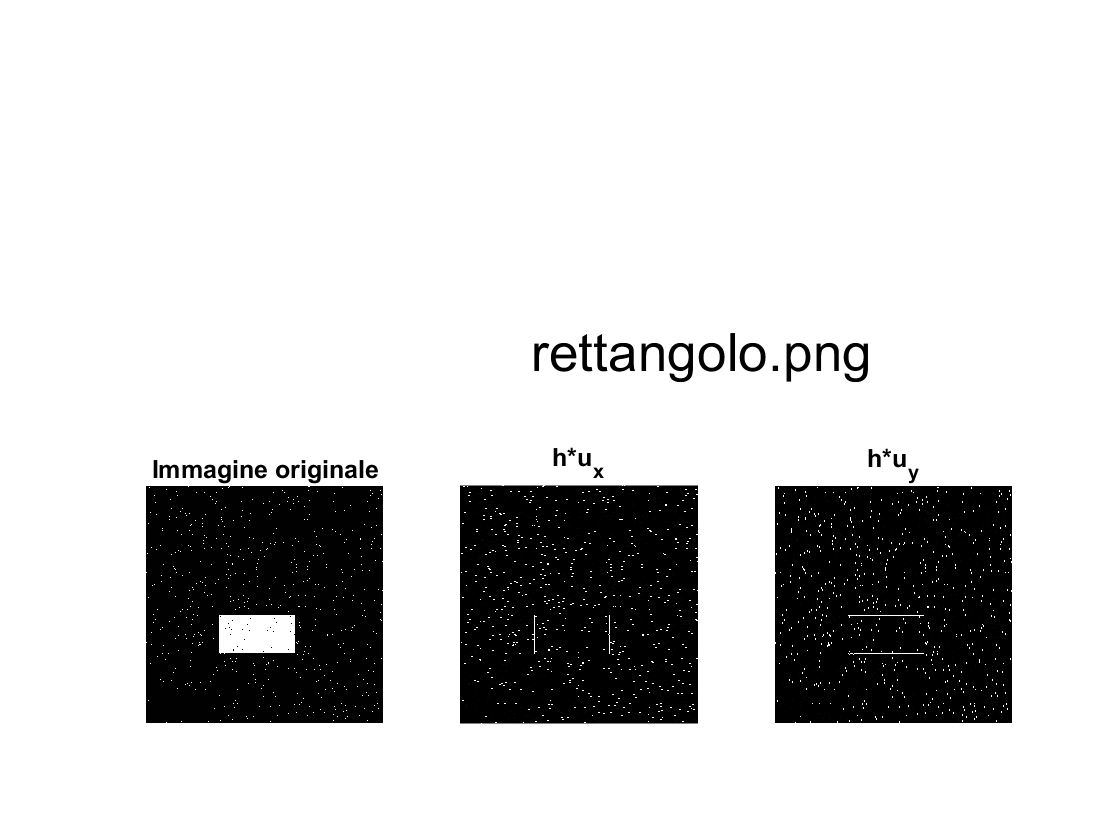
\includegraphics[scale=0.4, trim = 0 0 0 10.5cm, clip]{Pictures/Risultati/rettangolo bianco e nero derivate parziali con rumore.png}
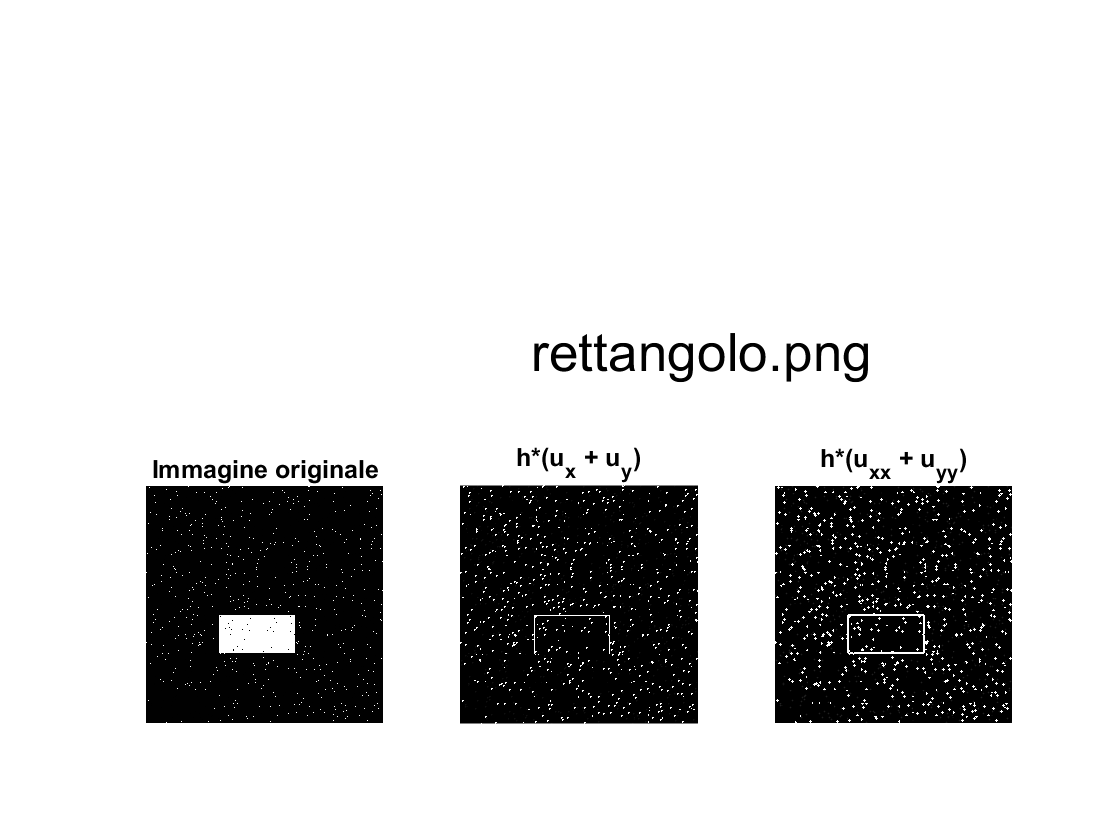
\includegraphics[scale=0.4, trim = 0 0 0 10.5cm, clip]{Pictures/Risultati/rettangolo bianco e nero gradiente e laplaciano con rumore.png}
\caption{Derivate parziali, gradiente e laplaciano di una figura semplice con rumore.}\label{fig:figura}
\end{figure}

Si può fare una considerazione: quando si trova un elemento di disurbo, come un puntino o una chiazza di colore, questo risulterà essere una forte variazione di colore improvvisa ed in quanto tale la derivata calcolata in un intorno di quel punto sarà, in valore assoluto, molto alta.
Questo vuol dire che il gradiente ne rileverà i bordi e il metodo Perona-Malik non lo toccherà, questa cosa non va bene: è un elemento di disturbo e va quindi eliminato.\\ 
Una possibile soluzione a questo problema verrà illustrata in seguito.\newpage


\newpage 
\subsection{Problema dei \textit{"bordi"} d'interferenza}
%\subsubsection{Considerazioni sui bordi}
%\subsubsection{Miglioramento dei bordi}
Come evidenziato con l'ultima immagine di prova nella sezione dedicata al rilevamento dei bordi, anche gli elementi di disturbo ne hanno e vengono quindi rilevati. Questo è un problema perché il metodo Perona-Malik tenderà a preservarli.\\
Per ovviare a questo problema operiamo su di una copia dell'immagine una diffusione come quella operata dall'equazione del calore vista in precedenza, così facendo in questa copia, i bordi dell'immagine risulteranno rovinati, ma non scomparsi! Gli elementi di disturbo saranno invece eliminati.\\
Moltiplicando i due gradienti così trovati si può osservare che: in corrispondenza degli elementi di disturbo il secondo gradiente sarà nullo ed il prodotto sarà dunque anch'esso nullo, vicino ai bordi il secondo gradiente non è nullo, ma il primo sì! Quindi il prodotto sarà ancora nullo, in corrispondenza degli effettivi bordi entrambi i gradienti saranno non nulli e quindi neanche il loro prodotto lo sarà. Questo vuol dire che:\\
\begin{itemize}
    \item gli elementi di disturbo sono stati eliminati
    \item l'effetto distruttivo sui bordi non viene riportato
    \item gli effettivi bordi dell'immagine vengono preservati
\end{itemize}
I bordi sono quindi calcolati in maniera efficiente.\\
\vspace{0em}
\subsubsection{La funzione di controllo}
\`E doveroso fare ancora una considerazione. Serve applicare ancora una trasformazione ai nostri bordi in modo da risultare ancor più efficienti ai nostri scopi, ossia una funzione di controllo. Cerchiamo una funzione decrescente tale che $k(0)=1$ e $\lim_{s\to\infty}k(s)=0$. Daremo in input a tale funzione il valore del gradiente calcolato in ogni pixel, otterremo così una mappatura che ci dice per ogni pixel in che misura operare la diffusione. Calato nel caso di studio, $k(0)=1$ vuol dire che dove non c'è bordo opera l'equazione del calore mentre $\lim_{|\nabla(u)|^2\to\infty}k(|\nabla(u)|^2)=0$ vuol dire che tanto più i bordi sono accentuati, tanto più l'equazione del calore non deve operare.
Facciamo questo banalmente perché considerando semplicemente i bordi, avremmo l'effetto opposto! Infatti dove non ci sono bordi $\nabla(u)=0$ e quindi non ci sarebbe diffusione, dove ci sono bordi molto marcati $\nabla(u)\to\infty$ quindi la diffusione verrebbe adoperata addirittura più del normale!
Non a caso una delle scelte più semplici, anche se non delle più classiche nè efficienti è $k=\frac{1}{1+|\nabla(u)|^2/c}$ dove c è un fattore di controllo.
Scelte decisamente più classiche ed impiegate sono:
\begin{itemize}
    \item $k=e^{-\frac{|\nabla(u)|^2}{c}}$ che preserva maggiromente i bordi ad altro constrasto e meno quelli a basso contrasto
    \item $k=\frac{1}{\sqrt{1+(|\nabla(u)|^2/c)}}$ che preserva maggiormente regioni grandi piuttosto che quelle piccole
\end{itemize} 
Come visto nella sezione 2.2.1 $div(k\nabla(u))=\frac{1}{2}(k_N\nabla_N + k_S\nabla_S k_W\nabla_W + k_E\nabla_E)$ calcoliamo quindi i vettori $k_N$, $k_S$, $k_W$ e $k_E$ dando in input alla funzione di controllo scelta i vettori $\nabla_N$, $\nabla_S$, $\nabla_W$ e $\nabla_E$ rispettivamente.

\newpage
\subsection{Implementazione}
Nel corso della trattazione sono stati forniti tutti gli elementi che portano alla formazione di questo script. Ci si limiterà quindi a dei richiami e a delle precisazioni di tipo tecnico.\\
\vspace{1em}
Prima di iniziare il filtraggio ci sono alcune operazioni preliminari da fare. In primo luogo occorrerà, ovviamente, caricare l'immagine che si intende filtrare. Successivamente l'immagine viene convertita in bianco e nero e viene aggiunto del rumore.\\
\begin{lstlisting}[language=MATLAB, name=listato]
img=imread('nome_file.png');            %Apertura dell'immmagine
img=rgb2gray(img);                      %Trasformazione in bianco e nero
im = imnoise(im,'salt & pepper',0.02);  %Aggiunta del rumore
\end{lstlisting}
\`E importante precisare che quest'ultima operazione, in un caso reale, non ha senso di esistere ma è messa lì per il puro scopo di simulare il problema che intendiamo risolvere.
\begin{lstlisting}[language=MATLAB, name=listato]
% conversione in double per il calcolo.
im = double(im);
\end{lstlisting}
Di norma codifichiamo le immagini come uint8 (interi senza segno da 0 a 255), tuttavia mantenere questa formattazione durante il calcolo potrebbe portare ad errori di approssimazione numerica assolutamente non trascurabili. Consideriamo quindi matrici a valori reali, approssimate dalla macchina a numeri macchina a doppia precisione. 
\begin{lstlisting}[language=MATLAB, name=listato]
% Condizioni iniziali della PDE.
diff_im = im;

num_iter=20;                            %numero di iterazioni
delta_t=0.1;                            %costante d'integrazione
c=60;                                   %coefficiente di controllo del                                       gradiente

sigma=1;                                %costante di controllo della                                         diffusione uniforme

\end{lstlisting}
Occorre settare alcuni parametri per il calcolo: 
\begin{itemize}
    \item Numero di iterazioni per il metodo di Eulero: maggiore è il valore di questo parametro e più volte verrà applicato il metodo
    \item Costante d'integrazione: maggiore è il valore di questo parametro e maggiore sarà l'intensità con cui viene applicato il metodo\\
    \vspace{0.25em}
    \textit{N.B. Sia aumentando il primo parametro sia il secondo ciò che otterremo sarà un'immagine filtrata maggiormente. La differenza è che aumentando la costante di integrazione applicheremo il metodo con maggior intensità ad ogni passo; invece aumentando il numero di iterazioni applicheremo il metodo un numero maggiore di volte. 
    Ad ogni iterazione tutti i calcoli andranno rifatti, ciò vuol dire che aumentando il numero di iterazioni e riducendo la costante di integrazione, avremo un'immagine filtrata più finemente a discapito di un grosso aumento di costo computazionale}
    \item Coefficiente di controllo del gradiente: permette di far risaltare di più (se c<1) o di meno (se c>1) i bordi
    \item costante di controllo diffusione uniforme: il calcolo del vettore c utilizzato per modificare l'equazione del calore avviene tramite gradiente. Come già analizzato nella sezione 5.3, conviene fare questo calcolo su una versione sfocata dell'immagine, per fare ciò applichiamo l'equazione del calore. Modificarne questo cofficiente significa modificare l'intensità con cui viene applicata. Un valore più alto sfoca di più e porta ad eliminare più rapidamente il rumore a discapito della definizione dei bordi.
\end{itemize}
Settati i parametri inizia il calcolo effettivo
\begin{lstlisting}[language=MATLAB, name=listato]

% Maschera di convoluzione
hN = [0 1 0; 0 -1 0; 0 0 0];
hS = [0 0 0; 0 -1 0; 0 1 0];
hE = [0 0 0; 0 -1 1; 0 0 0];
hW = [0 0 0; 1 -1 0; 0 0 0];


for t = 1:num_iter
   
    % Calcolo alle differenze finite nelle 4 direzioni
    nablaN = convoluzione(diff_im,hN);
    nablaS = convoluzione(diff_im,hS);   
    nablaW = convoluzione(diff_im,hW);
    nablaE = convoluzione(diff_im,hE);
    
    diff_blur = f_eq_del_calore(diff_im,delta_t,num_iter,sigma);
    nablaN_blur = convoluzione(diff_blur,hN);
    nablaS_blur = convoluzione(diff_blur,hS);   
    nablaW_blur = convoluzione(diff_blur,hW);
    nablaE_blur = convoluzione(diff_blur,hE);


    kN = exp(-(nablaN_blur/c).^2);
    kS = exp(-(nablaS_blur/c).^2);
    kW = exp(-(nablaW_blur/c).^2);
    kE = exp(-(nablaE_blur/c).^2);
\end{lstlisting}
Calcolati tutti i fattori possiamo in fine applicare il metodo utilizzando la formula trovata nella sezione 5.1
\begin{lstlisting}[language=MATLAB, name=listato]
    % Soluzione discreta della PDE.
    diff_im = diff_im + delta_t*(kN.*nablaN + kS.*nablaS + kW.*nablaW + kE.*nablaE );
          
\end{lstlisting}
Concludiamo stampando l'immagine rumorosa e quella filtrata per poter apprezzare gli effetti sortiti
\begin{lstlisting}[language=MATLAB, name=listato]
    % Stampa di controllo
    fprintf('\rIteration %d\n',t);
end
% Stampa dei risultati
figure('Name','Original picture');      %Stampa dell'immagine rumorosa
imshow(im);
figure('Name','Perona Malik');          %Stampa dell'immagine filtrata
imshow(uint8(diff_im));

\end{lstlisting}
